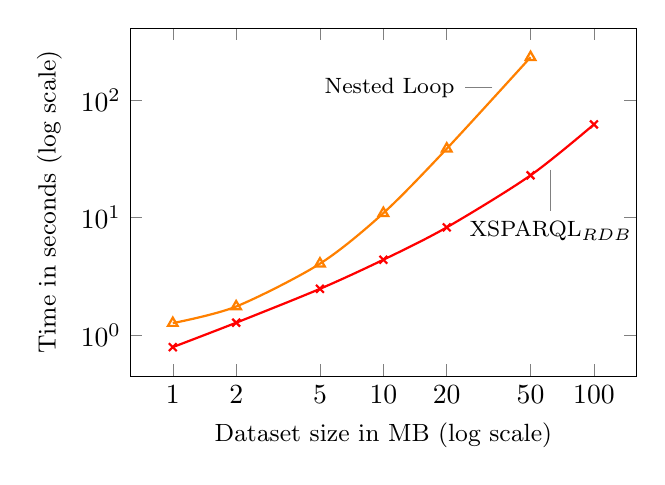
\begin{tikzpicture}[
]\begin{loglogaxis}[
xlabel={{\small Dataset size in MB (log scale)}},
ylabel={{\small Time in seconds (log scale)}},
scaled x ticks = false,
x tick label style = {/pgf/number format/fixed},
scaled y ticks = false,
y tick label style = {/pgf/number format/fixed},
xmax=100,enlargelimits=true,xtick={1,2,5,10,20,50,100},xticklabels={1,2,5,10,20,50,100},log basis x=10,log basis y=10,unbounded coords=jump,xminorticks=false,yminorticks=false,height=6cm,width=8cm,filter discard warning=false,legend style={inner sep=0,legend columns=2,draw=none,font=\tiny,at={(0,0)},anchor=south east,legend pos=south east,anchor=south east,legend cell align=left},pin distance=1em]


\addplot[thick,smooth, color=red, every mark/.append style={solid},mark=x,pin distance=1.5em] coordinates {
(1.0000000000, 0.7850000000)
(2.0000000000, 1.2687500000)
(5.0000000000, 2.4687500000)
(10.0000000000, 4.3725000000)
(20.0000000000, 8.2587500000)
(50.0000000000, 22.9437500000)
(100.0000000000, 62.4287500000)
} node[pos=.87,pin=-90:{\color{black}{{\footnotesize XSPARQL${}_{RDB}$}}}] {};;

\addplot[thick,smooth, color=orange, every mark/.append style={solid},mark=triangle,] coordinates {
(1.0000000000, 1.2587500000)
(2.0000000000, 1.7437500000)
(5.0000000000, 4.0475000000)
(10.0000000000, 10.9250000000)
(20.0000000000, 38.7450000000)
(50.0000000000, 233.7800000000)
(100.0000000000, NaN)
} node[pos=.9,pin=180:{\color{black}{{\footnotesize Nested Loop}}}] {};;


\end{loglogaxis}\end{tikzpicture}


%%% Local Variables:
%%% mode: latex
%%% mode: flyspell
%%% mode: reftex
%%% TeX-master: "../../presentation"
%%% End:
